\documentclass[11pt,a4paper]{article}
\usepackage{graphicx}

\title{Report of Kanji Assist}
\author{Witaut Bajaryn, Aleksander Mistewicz}

\begin{document}

\maketitle
\newpage

\section{Introduction}

We both attend japanese language classes. We noticed that there are services
offering translations, but not definition of a symbol or a group of them.
As we learn more kanji we would get help for chosen ones only.
There exist plugins that provide similar functionality, but they usually
work in a browser only.

We decided to design and implement an Android application that would
provide dictionary definition for anything that appears on a screen.

\section{Use example}

After the Kanji Assist first run (later: App) user is asked to select Kanji
Assistant as currently used Assitant in the Android system and is redirected
to said screen. User must agree to allow an App to read screen content.

After Kanji Assist is successfuly chosen it is ready to work. Assistant
is called with a long press of a Home button.

\begin{figure}[h]
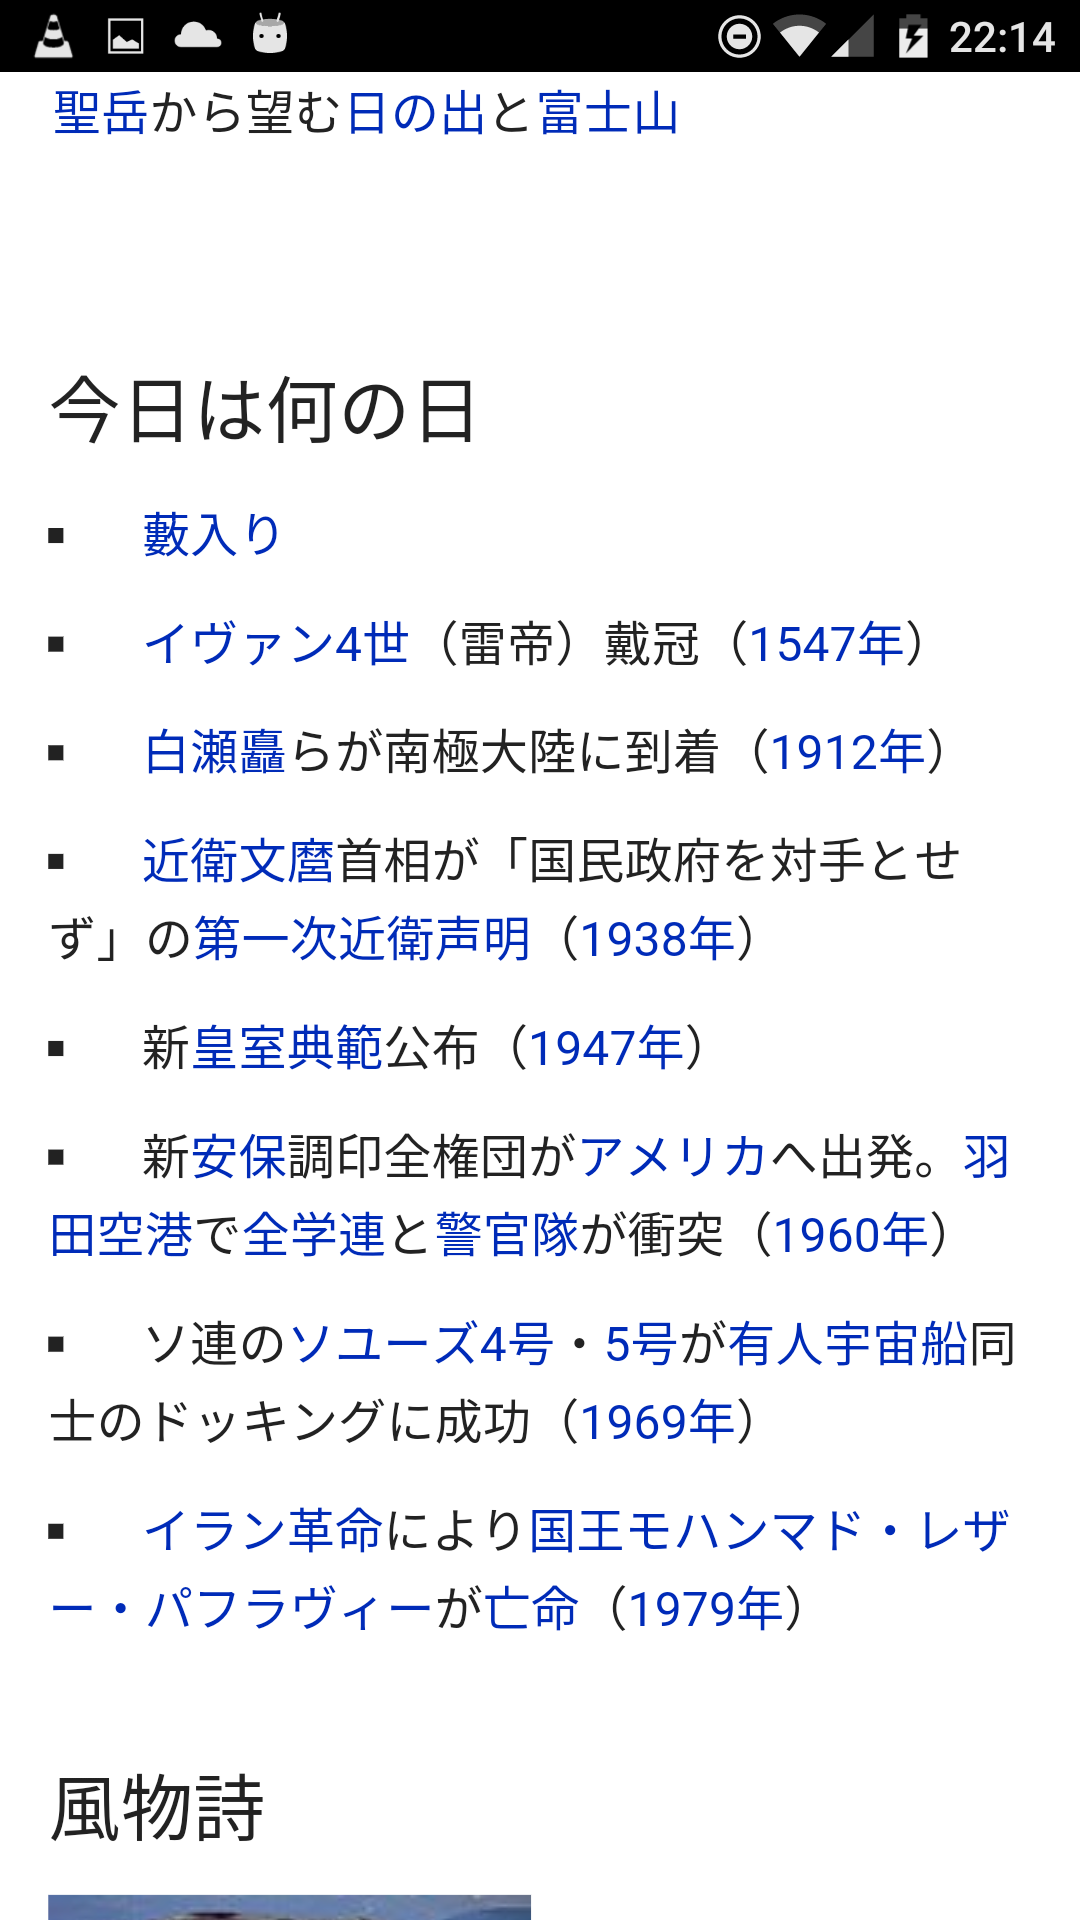
\includegraphics[width=110pt]{screen_3.png}
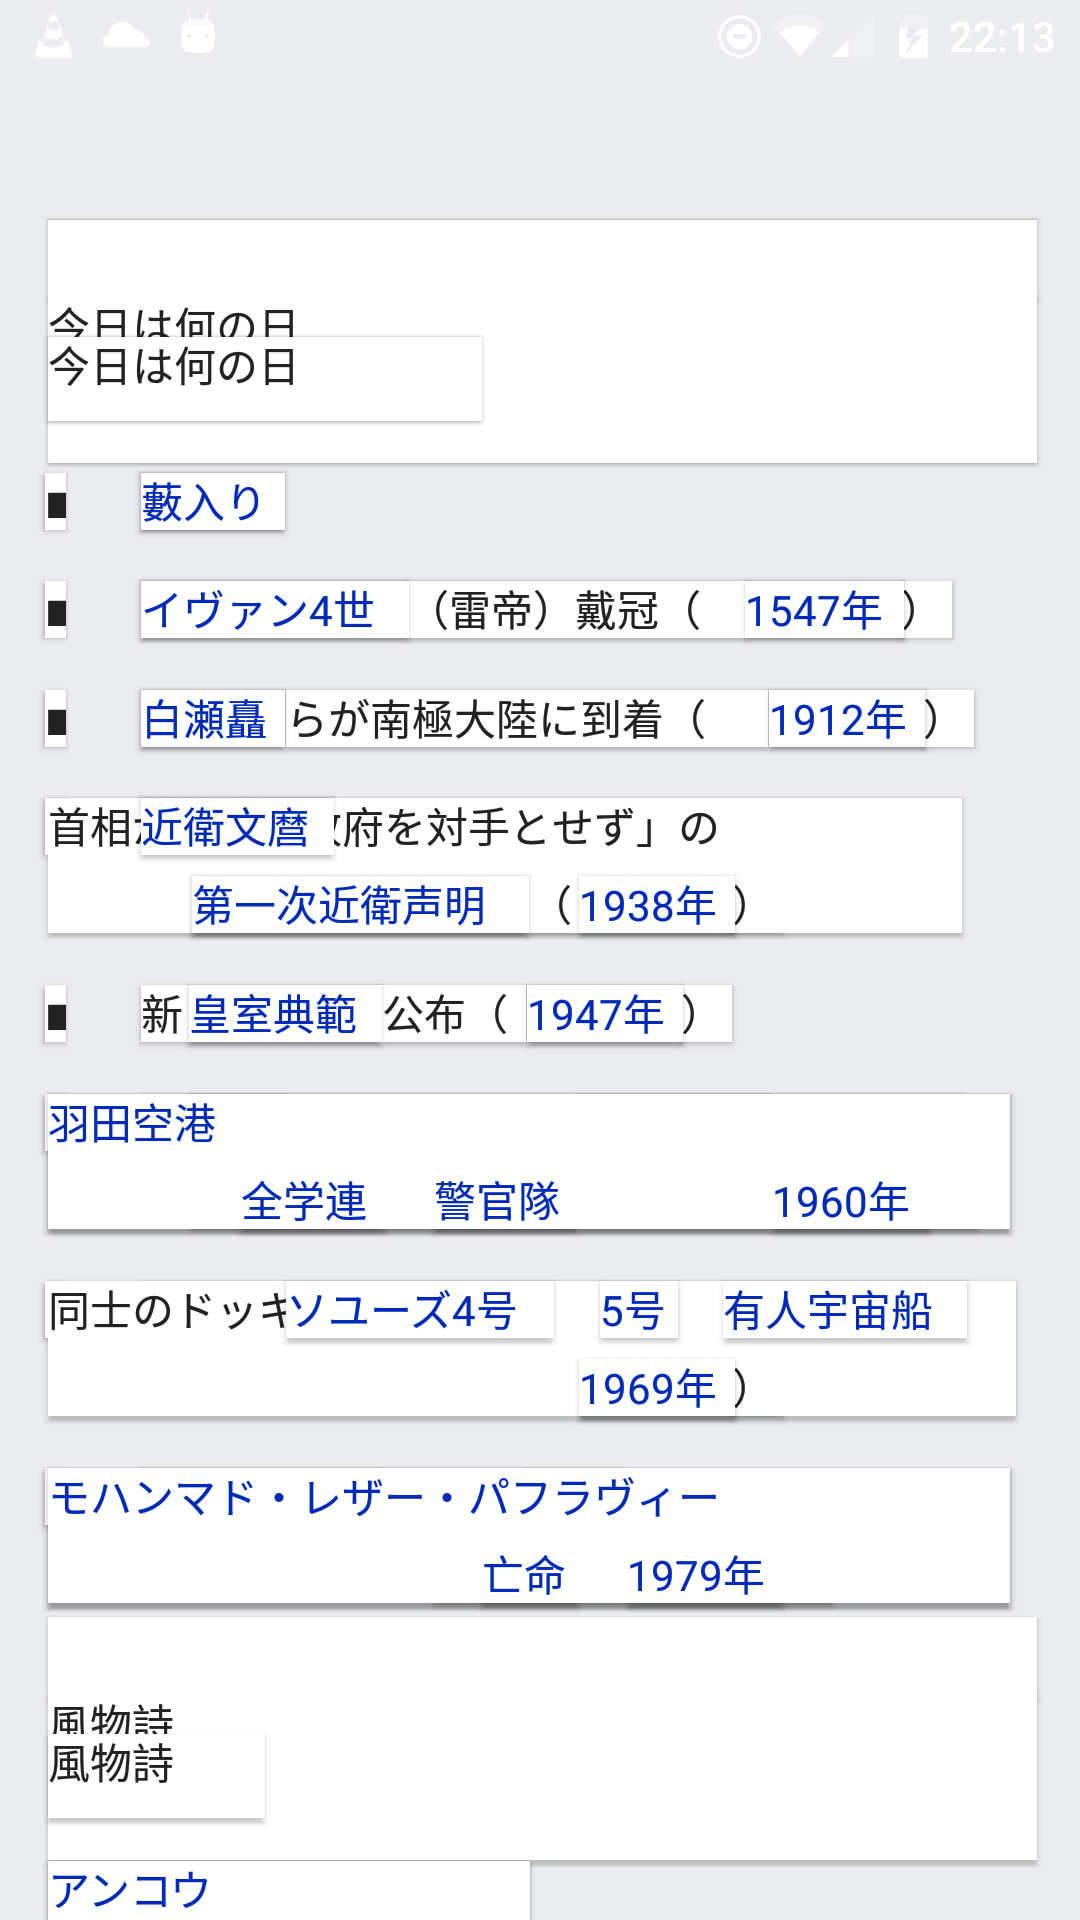
\includegraphics[width=110pt]{screen_1.png}
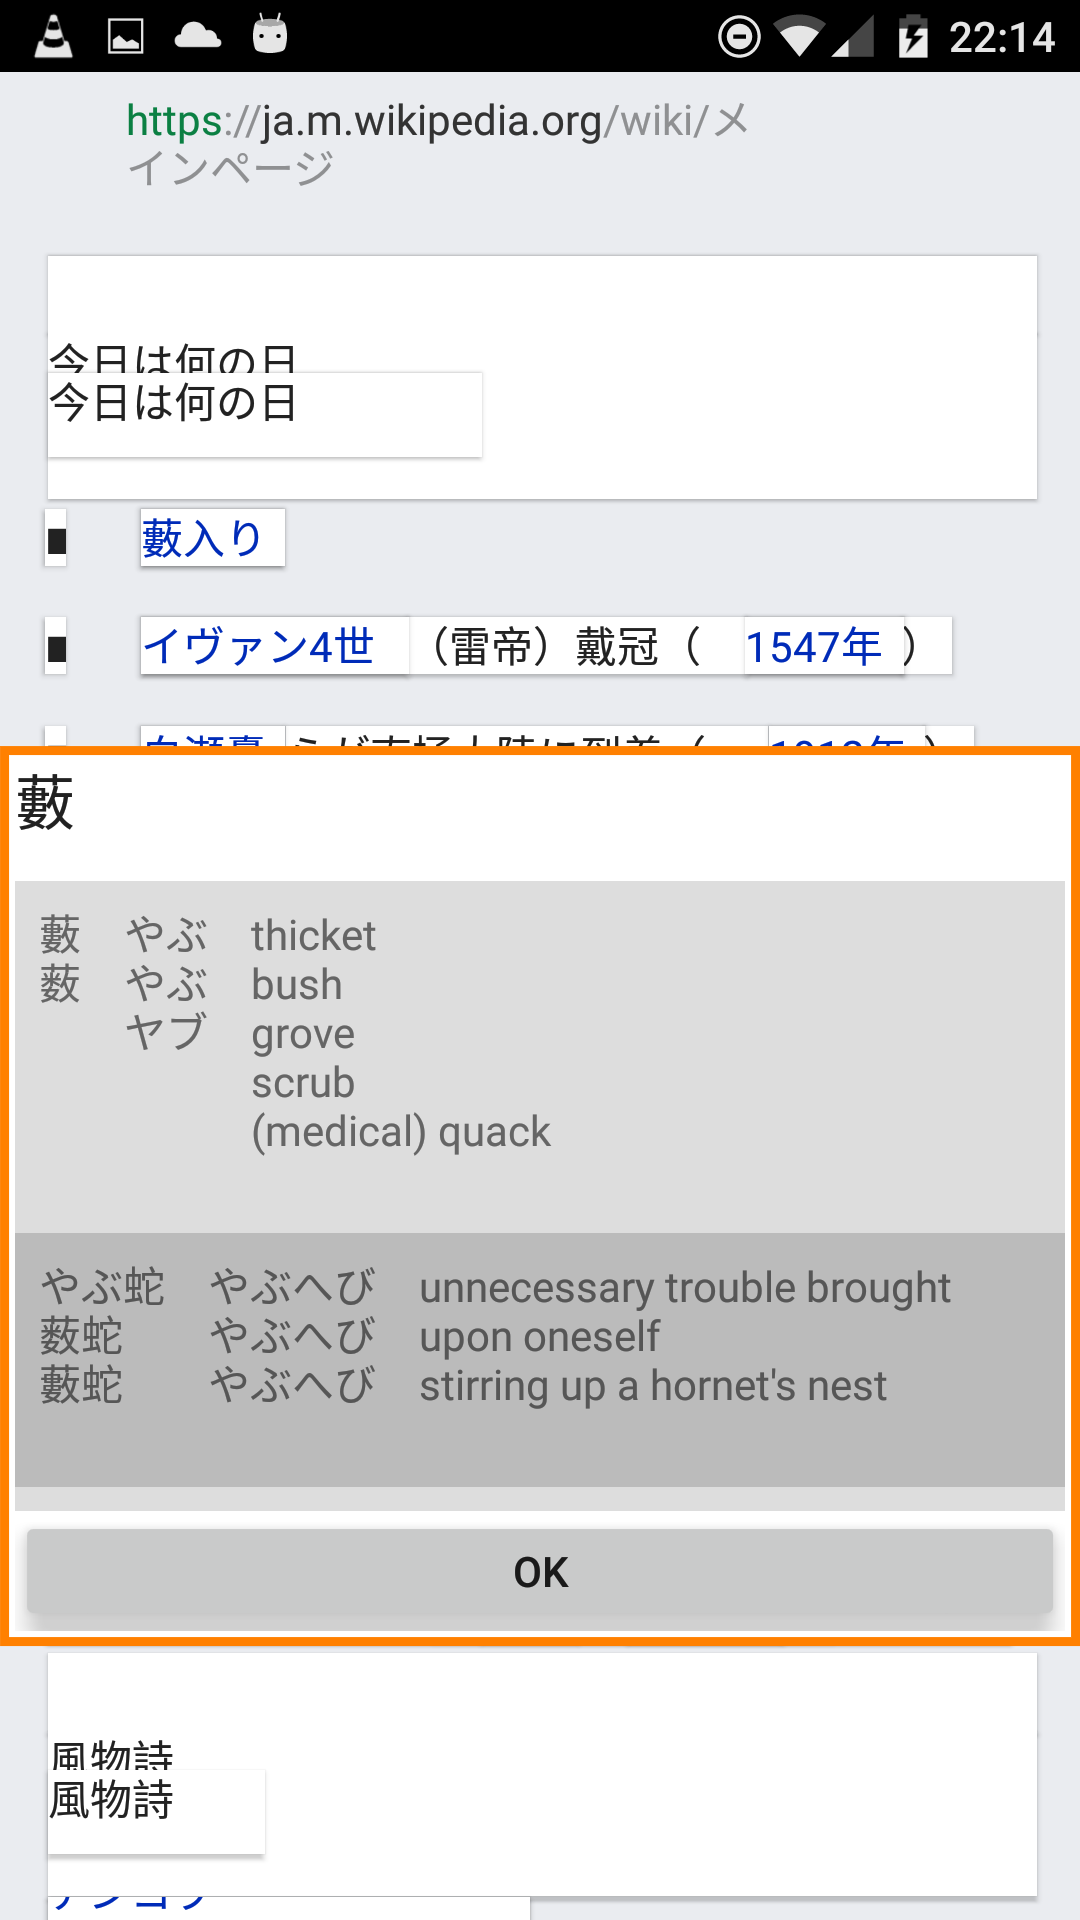
\includegraphics[width=110pt]{screen_2.png}

From the left: screen before Assistant is called, after Assitant's processing, after text selection
\end{figure}

Displayed content will be processed. If a text was selected, popup will appear.
Otherwise a user should long-press on text or double tap on view of interest
to get it.

Popup contains various examples of word use, reading and definition of a word
in english.

\newpage

\section{Future expansion}

Our plans for the future development include:
\begin{itemize}
    \item support for different dictionaries (including a local one)
    \item dictionary prefetching
    \item user customization: themes, information displayed
    \item ability to share query with a result to another app (e.g. Anki)
\end{itemize}

\section{Tests, problems}

During the course of our work we stumbled upon following issues:
\begin{itemize}
    \item Android's API for Asistant is not documented
    \item most Android testing frameworks do not support Assistant testing
    \item Assist Application implementation is not popular
    \item user can use only one Assistant at the time
\end{itemize}

\end{document}
